% Options for packages loaded elsewhere
\PassOptionsToPackage{unicode}{hyperref}
\PassOptionsToPackage{hyphens}{url}
%
\documentclass[
]{article}
\usepackage{amsmath,amssymb}
\usepackage{lmodern}
\usepackage{iftex}
\ifPDFTeX
  \usepackage[T1]{fontenc}
  \usepackage[utf8]{inputenc}
  \usepackage{textcomp} % provide euro and other symbols
\else % if luatex or xetex
  \usepackage{unicode-math}
  \defaultfontfeatures{Scale=MatchLowercase}
  \defaultfontfeatures[\rmfamily]{Ligatures=TeX,Scale=1}
\fi
% Use upquote if available, for straight quotes in verbatim environments
\IfFileExists{upquote.sty}{\usepackage{upquote}}{}
\IfFileExists{microtype.sty}{% use microtype if available
  \usepackage[]{microtype}
  \UseMicrotypeSet[protrusion]{basicmath} % disable protrusion for tt fonts
}{}
\makeatletter
\@ifundefined{KOMAClassName}{% if non-KOMA class
  \IfFileExists{parskip.sty}{%
    \usepackage{parskip}
  }{% else
    \setlength{\parindent}{0pt}
    \setlength{\parskip}{6pt plus 2pt minus 1pt}}
}{% if KOMA class
  \KOMAoptions{parskip=half}}
\makeatother
\usepackage{xcolor}
\usepackage[margin=1in]{geometry}
\usepackage{color}
\usepackage{fancyvrb}
\newcommand{\VerbBar}{|}
\newcommand{\VERB}{\Verb[commandchars=\\\{\}]}
\DefineVerbatimEnvironment{Highlighting}{Verbatim}{commandchars=\\\{\}}
% Add ',fontsize=\small' for more characters per line
\usepackage{framed}
\definecolor{shadecolor}{RGB}{248,248,248}
\newenvironment{Shaded}{\begin{snugshade}}{\end{snugshade}}
\newcommand{\AlertTok}[1]{\textcolor[rgb]{0.94,0.16,0.16}{#1}}
\newcommand{\AnnotationTok}[1]{\textcolor[rgb]{0.56,0.35,0.01}{\textbf{\textit{#1}}}}
\newcommand{\AttributeTok}[1]{\textcolor[rgb]{0.77,0.63,0.00}{#1}}
\newcommand{\BaseNTok}[1]{\textcolor[rgb]{0.00,0.00,0.81}{#1}}
\newcommand{\BuiltInTok}[1]{#1}
\newcommand{\CharTok}[1]{\textcolor[rgb]{0.31,0.60,0.02}{#1}}
\newcommand{\CommentTok}[1]{\textcolor[rgb]{0.56,0.35,0.01}{\textit{#1}}}
\newcommand{\CommentVarTok}[1]{\textcolor[rgb]{0.56,0.35,0.01}{\textbf{\textit{#1}}}}
\newcommand{\ConstantTok}[1]{\textcolor[rgb]{0.00,0.00,0.00}{#1}}
\newcommand{\ControlFlowTok}[1]{\textcolor[rgb]{0.13,0.29,0.53}{\textbf{#1}}}
\newcommand{\DataTypeTok}[1]{\textcolor[rgb]{0.13,0.29,0.53}{#1}}
\newcommand{\DecValTok}[1]{\textcolor[rgb]{0.00,0.00,0.81}{#1}}
\newcommand{\DocumentationTok}[1]{\textcolor[rgb]{0.56,0.35,0.01}{\textbf{\textit{#1}}}}
\newcommand{\ErrorTok}[1]{\textcolor[rgb]{0.64,0.00,0.00}{\textbf{#1}}}
\newcommand{\ExtensionTok}[1]{#1}
\newcommand{\FloatTok}[1]{\textcolor[rgb]{0.00,0.00,0.81}{#1}}
\newcommand{\FunctionTok}[1]{\textcolor[rgb]{0.00,0.00,0.00}{#1}}
\newcommand{\ImportTok}[1]{#1}
\newcommand{\InformationTok}[1]{\textcolor[rgb]{0.56,0.35,0.01}{\textbf{\textit{#1}}}}
\newcommand{\KeywordTok}[1]{\textcolor[rgb]{0.13,0.29,0.53}{\textbf{#1}}}
\newcommand{\NormalTok}[1]{#1}
\newcommand{\OperatorTok}[1]{\textcolor[rgb]{0.81,0.36,0.00}{\textbf{#1}}}
\newcommand{\OtherTok}[1]{\textcolor[rgb]{0.56,0.35,0.01}{#1}}
\newcommand{\PreprocessorTok}[1]{\textcolor[rgb]{0.56,0.35,0.01}{\textit{#1}}}
\newcommand{\RegionMarkerTok}[1]{#1}
\newcommand{\SpecialCharTok}[1]{\textcolor[rgb]{0.00,0.00,0.00}{#1}}
\newcommand{\SpecialStringTok}[1]{\textcolor[rgb]{0.31,0.60,0.02}{#1}}
\newcommand{\StringTok}[1]{\textcolor[rgb]{0.31,0.60,0.02}{#1}}
\newcommand{\VariableTok}[1]{\textcolor[rgb]{0.00,0.00,0.00}{#1}}
\newcommand{\VerbatimStringTok}[1]{\textcolor[rgb]{0.31,0.60,0.02}{#1}}
\newcommand{\WarningTok}[1]{\textcolor[rgb]{0.56,0.35,0.01}{\textbf{\textit{#1}}}}
\usepackage{graphicx}
\makeatletter
\def\maxwidth{\ifdim\Gin@nat@width>\linewidth\linewidth\else\Gin@nat@width\fi}
\def\maxheight{\ifdim\Gin@nat@height>\textheight\textheight\else\Gin@nat@height\fi}
\makeatother
% Scale images if necessary, so that they will not overflow the page
% margins by default, and it is still possible to overwrite the defaults
% using explicit options in \includegraphics[width, height, ...]{}
\setkeys{Gin}{width=\maxwidth,height=\maxheight,keepaspectratio}
% Set default figure placement to htbp
\makeatletter
\def\fps@figure{htbp}
\makeatother
\setlength{\emergencystretch}{3em} % prevent overfull lines
\providecommand{\tightlist}{%
  \setlength{\itemsep}{0pt}\setlength{\parskip}{0pt}}
\setcounter{secnumdepth}{-\maxdimen} % remove section numbering
\ifLuaTeX
  \usepackage{selnolig}  % disable illegal ligatures
\fi
\IfFileExists{bookmark.sty}{\usepackage{bookmark}}{\usepackage{hyperref}}
\IfFileExists{xurl.sty}{\usepackage{xurl}}{} % add URL line breaks if available
\urlstyle{same} % disable monospaced font for URLs
\hypersetup{
  pdftitle={RR-TB Updates},
  pdfauthor={Sarah Baum},
  hidelinks,
  pdfcreator={LaTeX via pandoc}}

\title{RR-TB Updates}
\author{Sarah Baum}
\date{2023-11-21}

\begin{document}
\maketitle

\hypertarget{model-specification}{%
\section{Model Specification}\label{model-specification}}

\hypertarget{overview}{%
\subsubsection{Overview}\label{overview}}

\begin{itemize}
\item
  State-level hierarchical generalized additive model (GAM) that models
  the prevalence of RR-TB positive cases per quarter among incident TB
  cases between 2014-2019
\item
  Fit smoothing functions to reduce the noise we were seeing in previous
  models
\item
  Models risk of positivity by characteristics of patient and
  municipality where they reside

  \begin{itemize}
  \tightlist
  \item
    Note: Between 2014-2019, \textasciitilde3,300 cases diagnosed
    outside of patient's state of residence; \textasciitilde88,000 cases
    diagnosed outside patient's municipality of residence (e.g.~cases
    are not being attributed to municipalities/states in which cases are
    generated)
  \end{itemize}
\item
  Separate models for new cases and previously treated cases
  (e.g.~relapse and re-entry)
\end{itemize}

\hypertarget{set-up}{%
\subsubsection{Set Up}\label{set-up}}

\begin{Shaded}
\begin{Highlighting}[]
\NormalTok{result }\SpecialCharTok{\textasciitilde{}} \FunctionTok{s}\NormalTok{(state, }\AttributeTok{bs =} \StringTok{"re"}\NormalTok{) }\SpecialCharTok{+} \FunctionTok{s}\NormalTok{(time) }\SpecialCharTok{+} \FunctionTok{s}\NormalTok{(time, }\AttributeTok{by =}\NormalTok{ state, }\AttributeTok{id =} \DecValTok{1}\NormalTok{) }\SpecialCharTok{+}\NormalTok{ age\_cat }\SpecialCharTok{+}\NormalTok{ hiv\_status }\SpecialCharTok{+}\NormalTok{ sex }\SpecialCharTok{+}\NormalTok{ health\_unit }\SpecialCharTok{+}\NormalTok{ bf\_cat }\SpecialCharTok{+}\NormalTok{ urban\_cat }\SpecialCharTok{+}\NormalTok{ has\_prison }\SpecialCharTok{+}\NormalTok{ fhs\_cat}
\end{Highlighting}
\end{Shaded}

\begin{itemize}
\item
  Random intercept for each state (patient state of residence)
\item
  A different smooth function for time by state with a shared smoothing
  parameter
\item
  Each state-level smoothing parameter varies around a grand smooth
  function for time to allow for pooling across states
\item
  Fixed effects for patient-level characteristics:

  \begin{itemize}
  \tightlist
  \item
    Age
  \item
    HIV status
  \item
    Sex
  \item
    Level of health unit where patient is diagnosed - Based on CNES
    merge
  \end{itemize}
\item
  Fixed effects for characteristics of region where patient resides
  (either municipality or micro-region level):

  \begin{itemize}
  \tightlist
  \item
    Urbanicity - Percent of the population in urban setting (2010
    census)
  \item
    Bolsa Familia coverage - Percent of the population benefiting from
    BF (BF: SAGICAD, 2018; Denominator: 2010 Census)
  \item
    Presence of prison - Municipality has prison at some point during
    2014-2019 period (SISPEN)
  \item
    FHS Coverage - Average number of health teams per 4,000 people
    between 2014-2019
  \end{itemize}
\end{itemize}

\hypertarget{specifications}{%
\subsubsection{Specifications}\label{specifications}}

\begin{itemize}
\item
  Model 1 - 2014-2019
\item
  Model 2 - 2016-2019
\item
  Run separately by case type (new vs.~previously treated (relapse,
  re-entry))
\end{itemize}

\hypertarget{model-output}{%
\section{Model Output}\label{model-output}}

\hypertarget{national-level-estimates}{%
\subsection{National-level estimates}\label{national-level-estimates}}

\begin{figure}
\centering
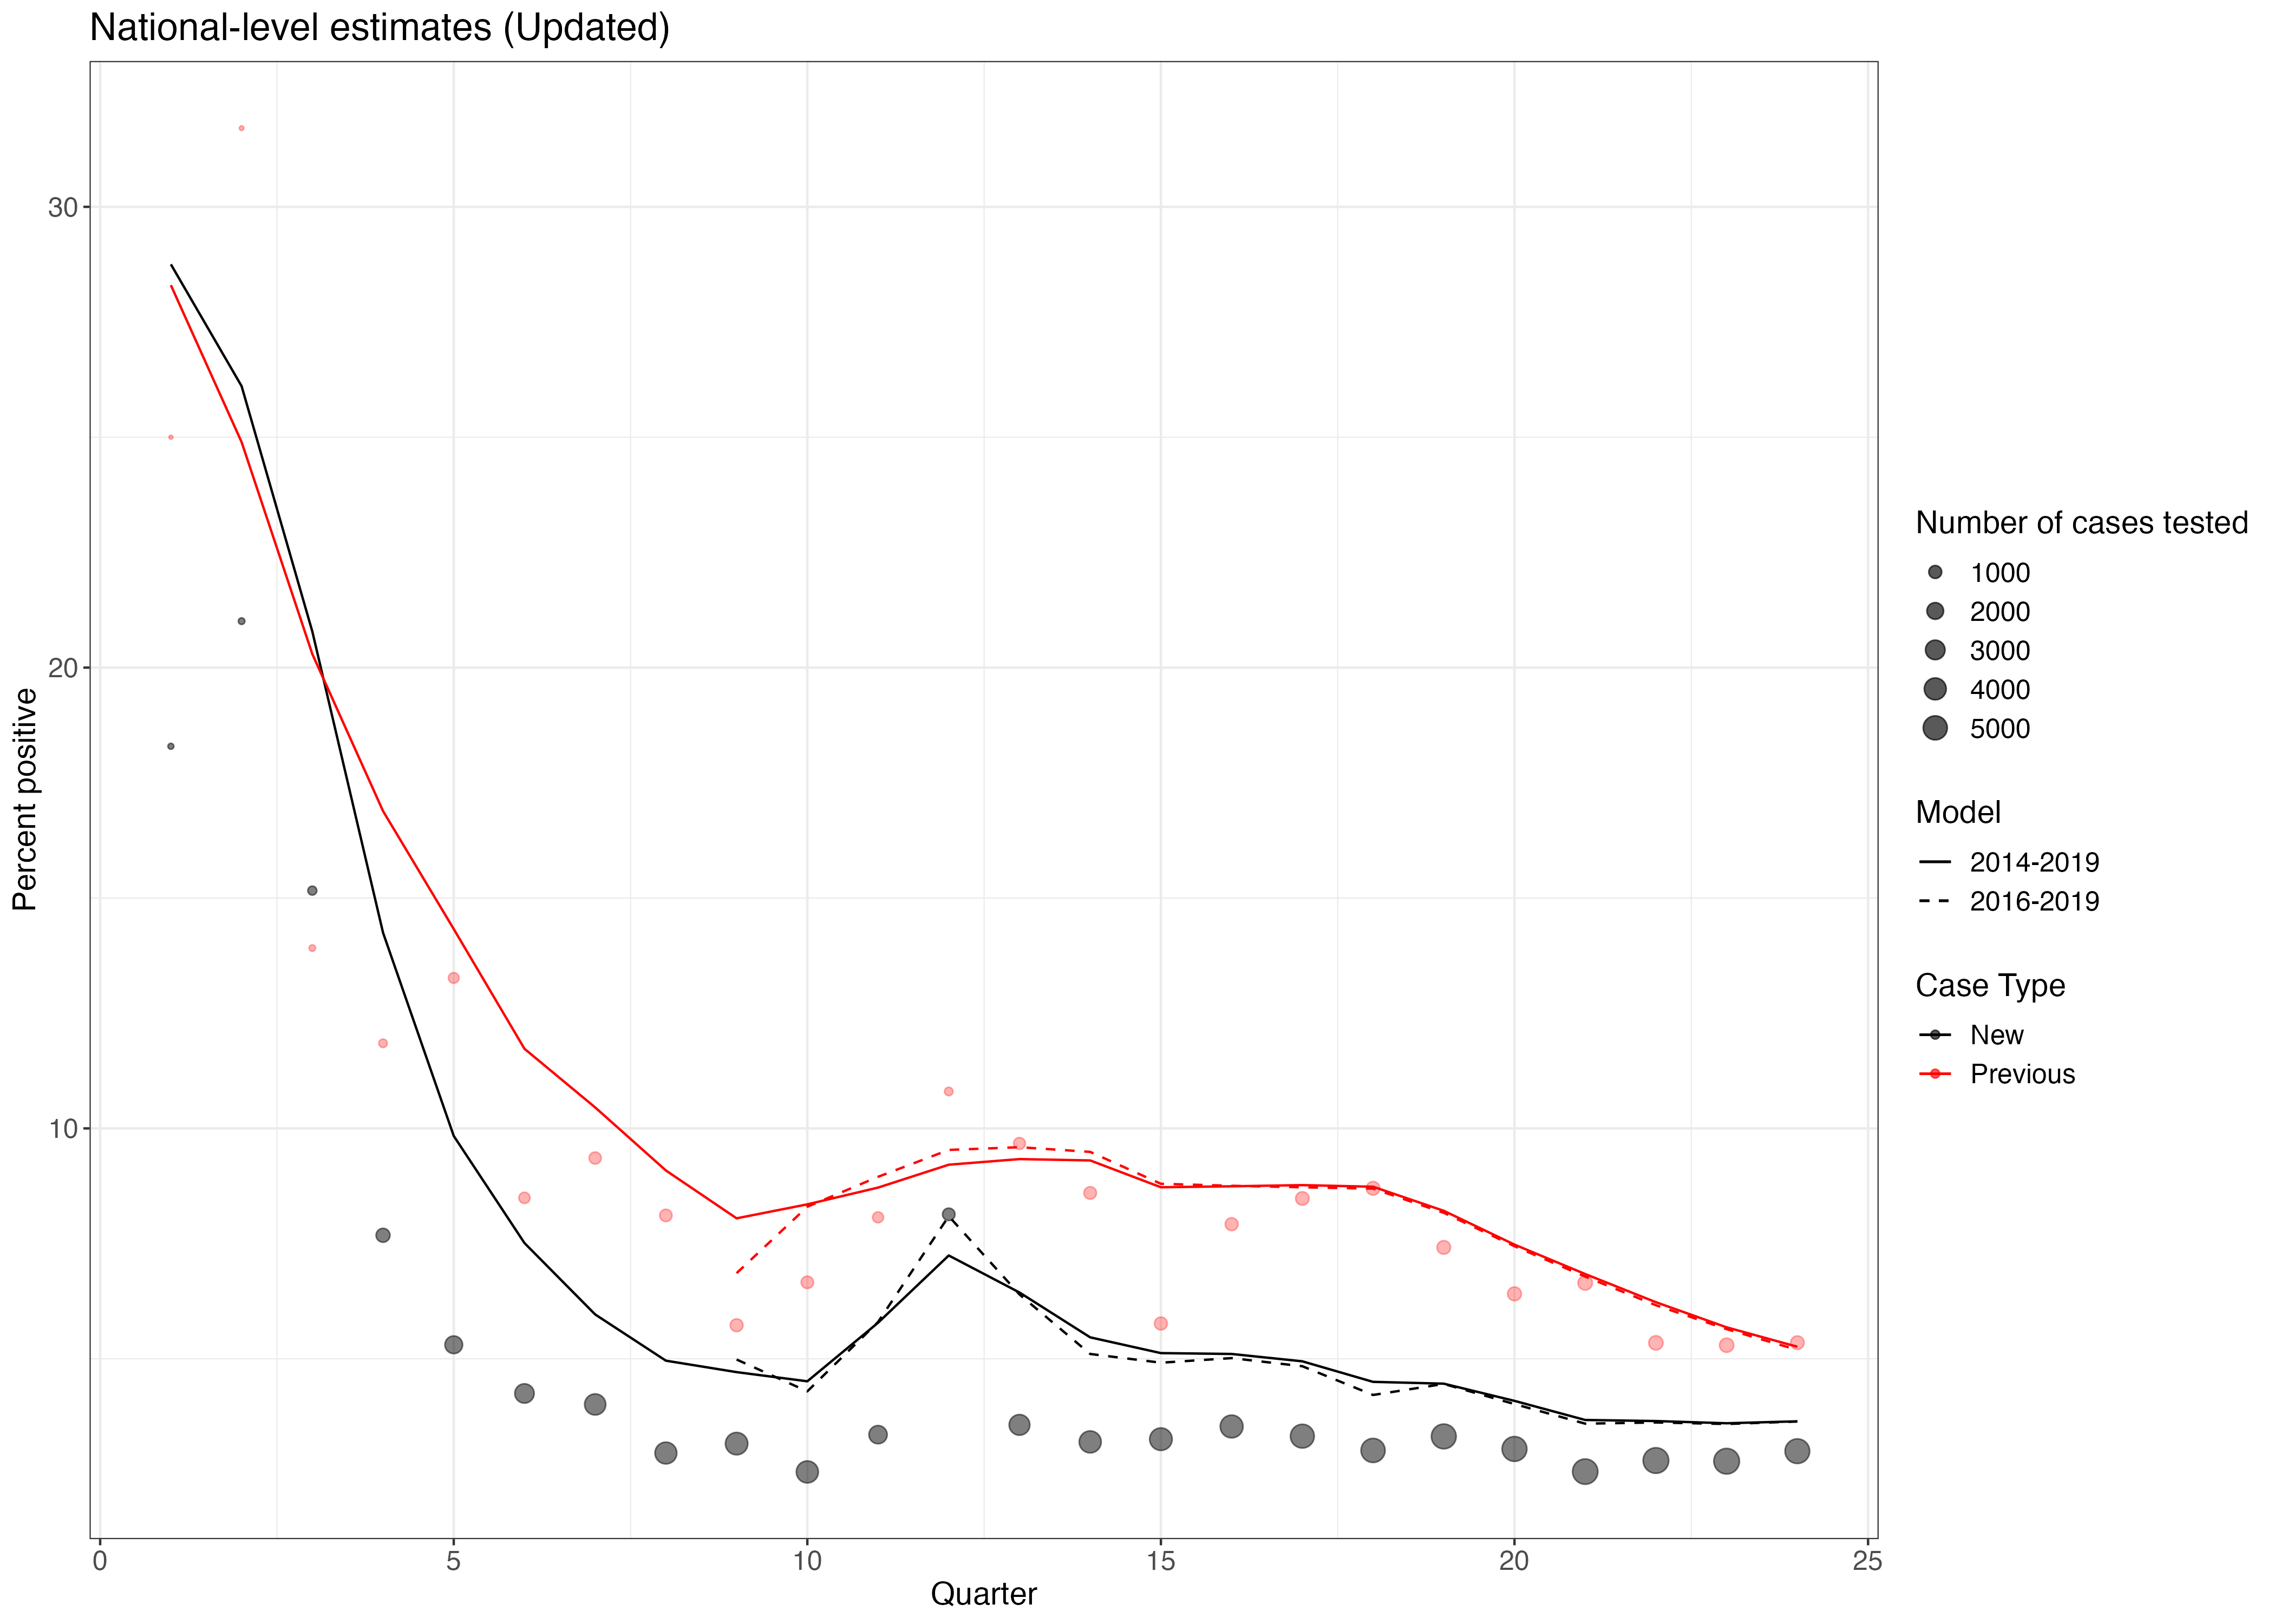
\includegraphics{Rif_Project/output/plots/plot_national_all.png}
\caption{caption}
\end{figure}

\end{document}
